
\begin{figure}[h]
  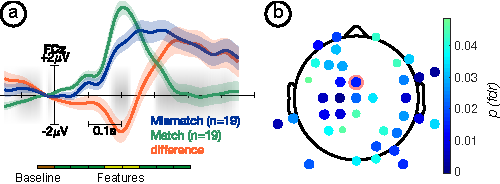
\includegraphics[width=.7\textwidth]{figures/erp_FCZ_diff_delay_with_scalp_map.pdf}
  \caption{\textcolor{n}{\textbf{a:}} Grand-average ERP (n = 19) of projected source mixtures at electrode FCz with significant class differences marked in grey. Bottom: Time windows used to compute features for classification (all greens). Windows in light green indicate time windows of interest for classifier source localization. \textcolor{n}{\textbf{b:} Electrodes with a significant amplitude difference (\textit{fdr} corrected) between match and mismatch trials at 200 ms post tap event. Electrode locations are color scaled by their respective p-value, colder colors correspond to a lower p-value. Scalp location of electrode FCz (see subplot \textbf{a}) is highlighted with a red background.}}
  \label{erp}
\end{figure}

\subsection{$\sim$77 \% Classification Accuracy Detecting VR Glitches using ERPs}

We found significant differences between match and mismatch trials in the grand-average event-related potential (ERP) at several scalp locations, see figure \ref{erp} showing the ERP at electrode `FCz' for an example. Hence, we reproduced our previous findings in \cite{Gehrke2019-og} with an altered processing pipeline. At electrode `FCz', amplitude differences at 200 ms indicated a significant difference between mismatch, i.e. the VR glitch condition and the matching trials ($t_{18} = -5.34, p < .001$). Differences were observed most strongly in the 150-280 ms time window, at 250 ms and in later windows starting at 350 ms, see figure \ref{erp}.

To assess the potential for single-trial online applications, a discriminative classification system was cross-validated. The system, using windowed mean ERP features, succeeded in detecting VR glitches. Mismatch and match trials were correctly labeled to the corresponding class with an average accuracy of $\sim$77 percent ($SD = 9.12$). The classification accuracy exceeded chance level at $\sim$ 56 percent, $t_{(18)} = 42.1, p < .001$. 

\subsubsection{Classification Driven by Midline Cingulate and Occipital EEG Sources}

To draw conclusions about the cortical origin of the discriminatory signal we investigated which EEG sources contributed maximally to the classification. With regards to the system's applicability as robust neural interface technology, this source reconstruction served two purposes: (1) Asserting that the classifier did not rely \textit{primarily} on artifact EEG sources, and (2) to gain additional information about the contributing brain regions to allow interpretations about cognitive processing.

In the fourth time window of the eight windowed mean features (150 - 200 ms, see the first light green shaded window at the bottom of figure \ref{erp} and in figure \ref{lda_loc}a top) classifications were driven primarily by activity originating in right lateral parieto-occipital cortical sources (BA19; MNI: x = 30, y = -70, z = 30), see figure \ref{lda_loc}a bottom. In the following time-window (200 - 250 ms, see the second light green shaded window at the bottom of figure \ref{erp} and in figure \ref{lda_loc}b top) the classification signal draw from distributed source activity in occipital areas as well as from sources located in anterior midline cingulate gyrus (near BA23; MNI: x = 0, y = -10, z = 30), see figure \ref{lda_loc}b bottom. Some ocular sources were not classified as such by our automated processing pipeline and carried information relevant to classification in this time window of interest.

\begin{figure}[!h]
  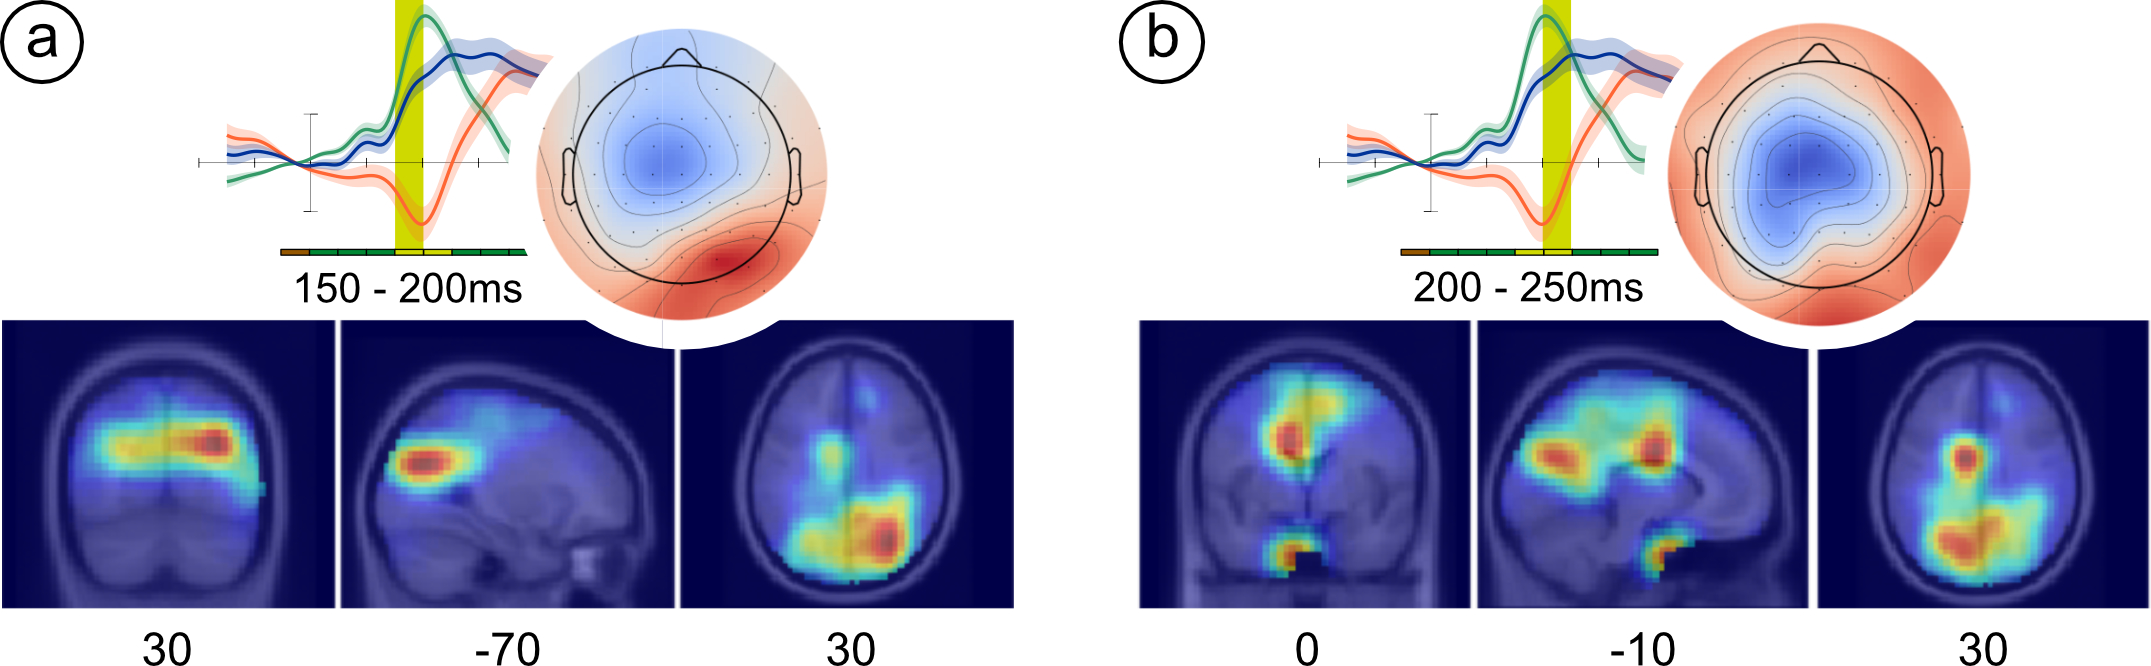
\includegraphics[width=\textwidth]{figures/fig_localization.jpg}
  \caption{An LDA classifier was trained on eight windowed means of 50 ms size from 0 to 400 ms following the cube tap, see figure \ref{erp} bottom. Two classes of synchronous and asynchronous trials were labeled for training and cross-validation. \textbf{a, b} Scalp maps of difference-between-classes activity for the 4th (150-200) and 5th (200-250ms) time windows and the equivalent source localization (MNI coordinates of the location of maximum activity).}
  \label{lda_loc}
\end{figure}